\subsection{Wellenlänge}
Berechnen sie die Frequenz einer Radiowelle mit der Wellenlänge $\lambda$ von 5$00m$
\[
	f=\frac{c}{\lambda} = \frac{3\cdot 10^8m/s}{500 m} = 600kHz
\]

Ein Laser mit einer Frequenz von $4.5\cdot 10^{14} Hz$ und einer Leistung von $P=0.2mW$ sendet Photonen aus. Wieviele Photonen verlasen den Laser pro Sekunde.
\begin{itemize}
\itemsep0em
\item $h = $ Planksches Wirkungsquantum $=6.6\cdot 10^{-34}\frac{J}{Hz} = 6.6\cdot 10^{-34} Js$
\item $n = $ Anzahl Photonen
\end{itemize}
\begin{align*}
E= h\cdot f\\
E_{ges} &= n\cdot E\\
P&= \frac{E_{ges}}{t} = \frac{E\cdot n}{t}\\
n&=\frac{P\cdot t}{E\cdot n} = \frac{0.0002W\cdot 1s}{6.6\cdot 10^{-34}Js\cdot 4.5\cdot10^{14}Hz} \approx 6.7\cdot 10^{14}
\end{align*}

\subsection{Lichtbrechung}
Ein gelber Lichtstrahl mit einer Wellenlänge von $\lambda = 589 nm$ trifft unter einem Einfallswinkel $\alpha_1 = 25^\circ$ auf die Grenzfläche zwischen Wasser und Flintglas. Unter welchem Winkel wird
er von seiner ursprünglichen Richtung abgelenkt? Die Brechungsindizes bei $\lambda = 589 nm$ betragen:\\
\begin{tabular}{ll}
Wasser: &$n = 1.333$\\
Flintglas: &$n = 1.603$
\end{tabular}


\begin{minipage}{0.69\textwidth}
\begin{align*}
	\delta &= \varepsilon_1-\varepsilon_2\\
	n_1\cdot \sin(\varepsilon_1) &= n_2\cdot \sin(\varepsilon_2)\\
	\delta &= \varepsilon_1 - \arcsin\left(\frac{n_1}{n_2}\cdot \varepsilon_1\right)\\
	4.42^\circ&=-\arcsin\left(\frac{1.333}{1.603}\cdot \sin(25^\circ)\right)
\end{align*}
\end{minipage}
\begin{minipage}{0.3\textwidth}
	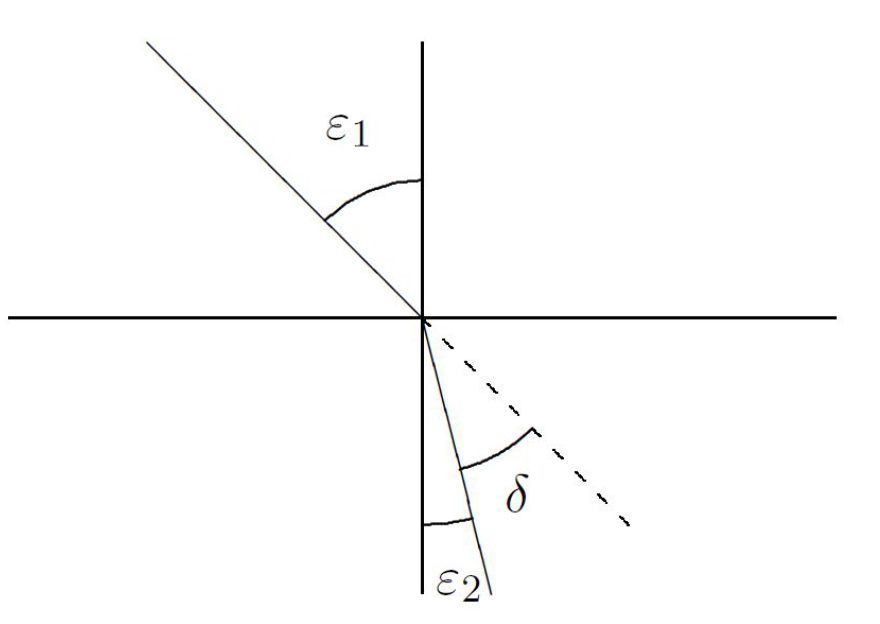
\includegraphics[width=0.9\textwidth]{bilder/lichtbrech.png}
\end{minipage}

\textbf{Spiegel}\\
Wie gross ist das Bild eines 4 cm grossen Gegenstands, der sich im Krümmungsmittelpunkt eines sphärischen Konkavspiegels mit einem Krümmungsradius von 50 cm befindet? Wie gross ist die Bilddistanz?
\[
	f=\frac{r}{2} = 0.25m\quad \frac{1}{f} = \frac{1}{b}+\frac{1}{g} \qquad b= \frac{1}{\frac{1}{f}-\frac{1}{g}} = \frac{1}{\frac{1}{0.25}- \frac{1}{0.5}} = 0.5m \qquad \frac{B}{G} = \frac{b}{g} \Rightarrow B= \frac{b\cdot G}{g} = \frac{0.5\cdot 0.04}{0.5} = 0.04m = 4cm
 \]
Wobei: \begin{itemize}
			\itemsep0em
			\item $f$ = Brennweite
			\item $g$ = Gegenstandsweite (Abstand vom Spiegel zum Gegenstand)
			\item $b$ = Bildweite (Abstand vom Spiegel zum Bild)
			\item $B$ = Bildgrösse
			\item $G$ = Gegenstandsgrösse
\end{itemize}

\textbf{Kamera und Spiegel}
Ein Fotoamateur fotografiert in einem Reisebus Personen der Reisegesellschaft über den Innenrückspiegel des Fahrers. Die Kamera ist $1m$ vom Rückspiegel entfernt. Um das Bild von Passagieren, die sich 1.5 m hinter der Kamera befinden, scharf zu erhalten, muss der
Amateur das Objektiv auf eine Distanz von 1.8 m einstellen. Wie gross ist die Brennweite des Rückspiegels?

\begin{minipage}{0.39\textwidth}
\[
	b = a-d =-0.8m\qquad g = a+c = 2.5m
\]
\[
	f=\frac{1}{\frac{1}{g}+\frac{1}{b}} = \frac{1}{\frac{1}{2.5m}+\frac{1}{(-0.8m)}} = -1.18m
\]
\end{minipage}
\begin{minipage}{0.59\textwidth}
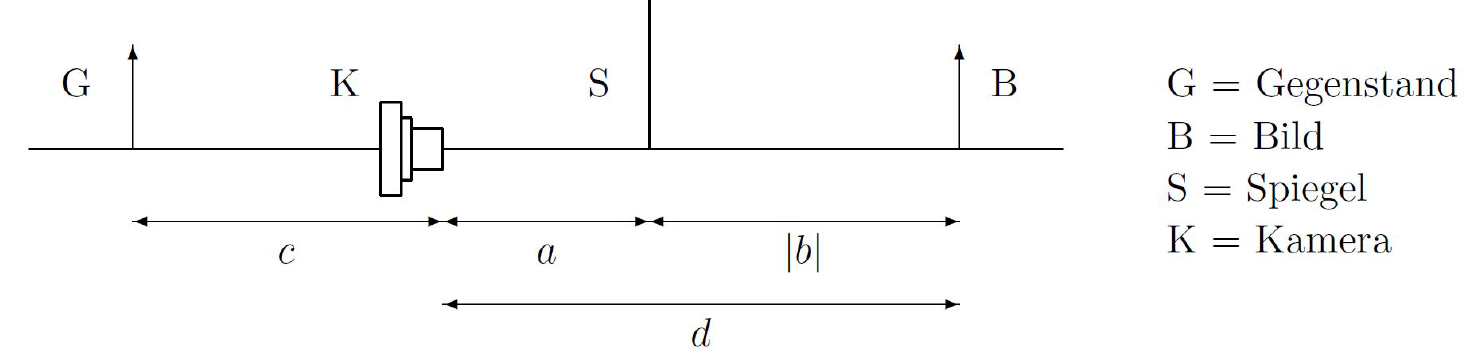
\includegraphics[width=0.99\textwidth]{bilder/a31.png}
\end{minipage}

\textbf{Kamera I}\\
Ein Fotoobjektiv mit einer Brennweite von 50 mm ist in einer Gewindefassung mit einer Ganghöhe von 4 mm in eine Kamera eingebaut. Wie gross ist der Drehwinkel zwischen
den Entfernungseinstellmarken für 3 m und 5 m?
\[
	\Delta b = b_1-b_2 = \left(\frac{1}{\frac{1}{f}-\frac{1}{g_1}}-  \frac{1}{\frac{1}{f}-\frac{1}{g_2}}\right) = \left(\frac{1}{\frac{1}{0.05}-\frac{1}{3}}-\frac{1}{\frac{1}{0.05}-\frac{1}{5}}\right) = 0.3424mm\qquad \alpha = \frac{\Delta b}{h} \cdot 360^\circ = \frac{0.3424mm}{4mm}\cdot 360^\circ = 30.81^\circ
\]

\textbf{Kamera mit Unschärfe}\\
Ein Fotoamateur will einen Motorradfahrer, der mit einer Geschwindigkeit von $v=72 km/h$ vorbeifährt, aus $g=10m$ Distanz von der Seite fotografieren. Sein Fotoapparat hat ein
Objektiv mit $f=50 mm$ Brennweite. Welche Belichtungszahl muss er einstellen, damit die
Bewegungsunschärfe auf dem Film höchstens 0.1 mm wird?\\
Die Bewegungsunschärfe kann als Bildgrösse $B$ interpretiert werden!
\begin{align*}
	b&= \frac{1}{\frac{1}{f}-\frac{1}{g}} \textrm{ da f }<< g \Rightarrow b\approx f\\
	G&= \frac{g\cdot B}{b} \quad \textrm{und} \quad G=v\cdot t \quad \Rightarrow v\cdot t = \frac{g\cdot B}{b}\\
	t&= \frac{g\cdot B}{f\cdot v} = \frac{10m \cdot 0.1mm}{0.05mm \cdot 20m/s}= \frac{1}{1000}s
\end{align*}

\textbf{Kamera mit Unschärfe II}\\
Das $f=35mm$ Objektiv eines Fotoapparates ist auf $g_0= \infty$ eingestellt. Wie nahe darf ein Gegenstand sein, damit bei einer Blendenöffnung von $q=1/16$ die Unschärfe des Bildes kleiner als $2\cdot 10^{-5}$m ist?
\begin{align*}
\frac{1}{g} &= \frac{1}{g_0} \pm \frac{u}{qf^2}  \\
g&=\frac{1}{\frac{1}{g_0} \pm \frac{u}{qf^2}} \quad \textrm{da }g_0= \infty \Rightarrow g= \frac{qf^2}{u} = \frac{1\cdot (0.035)^2}{16\cdot 2\cdot 10^{-5}} = 3.828m
\end{align*}

\textbf{Fernrohr}
Ein Turm von 40 m Höhe wird aus einer Entfernung von $g=12km$ durch ein astronomisches Fernrohr betrachtet, dessen Objektiv eine Brennweite $f_1=150cm$ und dessen Okular eine Brennweite $f_2=5 cm$ aufweist. Welche Distanz müssen die beiden Linsen voneinander
haben, wie gross ist die Vergrösserung, und unter welchem Sehwinkel erscheint der Turm im Fernrohr? Wie gross ist die Austrittspupille, und in welchem Abstand vom Okular befindet sie sich, wenn das Fernrohr eine Lichtstärke von $L=25$ aufweist? Wie gross ist der
Durchmesser des Objektivs?

\begin{align*}
l &= f_1+f_2 = 150cm+5cm = 155cm\\
V &= \frac{f_1}{f_2} =\frac{150}{5} = 30\\
\varepsilon&= \arctan\left(\frac{B}{f_2}\right) \quad B = \frac{b\cdot G}{g}\quad b= \frac{1}{\frac{1}{f_1}-\frac{1}{g}} \approx f_1\\ 
\varepsilon&= \arctan\left(\frac{f_1\cdot G}{g\cdot f_2}\right) = \arctan\left(\frac{1.5\cdot 40}{12'000\cdot 0.05}\right) = 5.71^\circ
\end{align*}



